\subsection{集群运行}
\subsection{PageRank词云}
根据PageRank的结果,按照人物的PR值大小生成词云,可以直观的看出哪些人物是主角。
		\begin{figure}[ht]
			\centering
			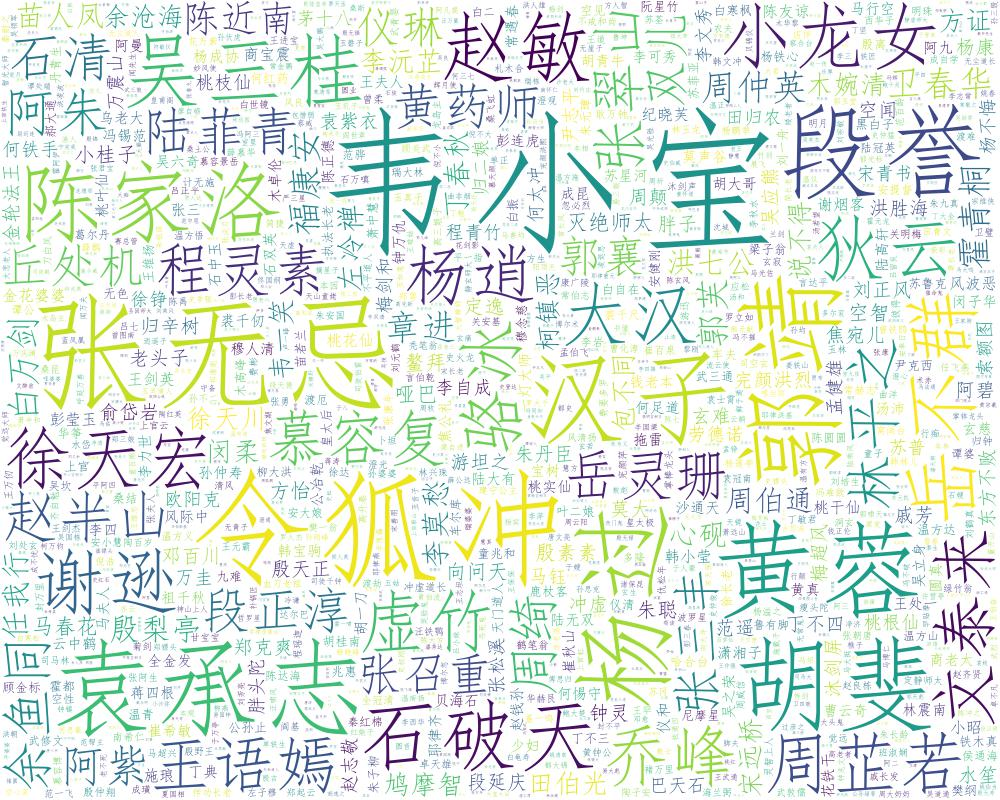
\includegraphics[scale=0.38]{figures/wordcloud.jpg}
			\caption{根据PageRank值生成词云}
		\end{figure}
\subsection{标签传播聚类}
根据PageRank和标签传播的结果,对人物关系图进行染色,可以看出哪些人物之间的关系密切,哪些人物属于同一本书。
\begin{figure}[ht]
	\centering
	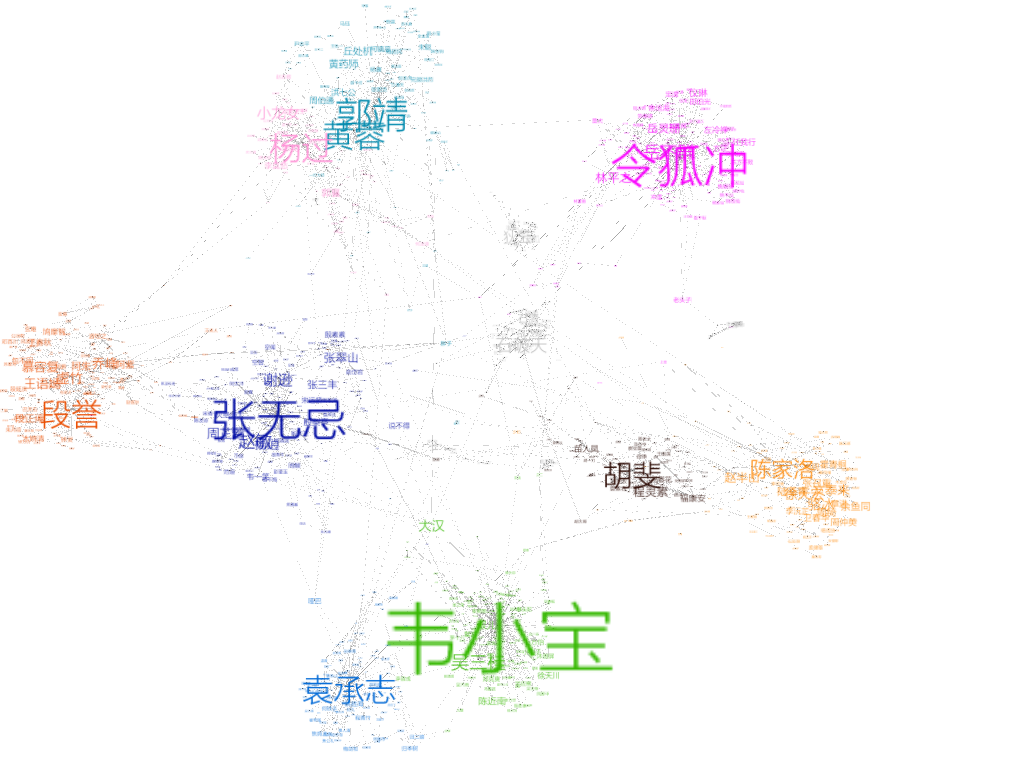
\includegraphics[scale=0.45]{figures/label_prop.png}
	\caption{标签传播结果可视化}
\end{figure}